% -*- TeX -*-

\documentclass{beamer}
\usepackage{amsmath}

\title{Crustal Deformation Modeling Tutorial}
\subtitle{Meshing Strategies}
\author{Charles Williams, Brad Aagaard, and Matthew Knepley}
\institute{\includegraphics[scale=0.4]{../../logos/cig_blackfg}}
\date{June 24, 2013}


% ---------------------------------------------------- CUSTOMIZATION
\renewcommand{\thispdfpagelabel}[1]{}
\newcommand{\important}[1]{{\color{red}#1}}
\usetheme{CIG}

% --------------------------------------------------------- DOCUMENT
\begin{document}

% ------------------------------------------------------------ SLIDE
\maketitle

% ========================================================== SECTION
\section{Meshing}
\subsection{General steps}

% ------------------------------------------------------------- LOGO
\logo{\includegraphics[height=4.5ex]{../../logos/cig_blackfg}}

% ------------------------------------------------------------ SLIDE
\begin{frame}
  \frametitle{Meshing Complex Geometry}
  \summary{Steps in creating a mesh}
  
  \begin{itemize}
  \item Determine geometric features needed
    \begin{itemize}
    \item Fault geometry
    \item Topography
    \item Sharp structural boundaries
    \item Magma sources with complex geometry
    \end{itemize}
  \item Create spline curve (2D) or NURBS surface (3D) in CUBIT
  \item If using surface in several models export it for future use
  \item Use surfaces within CUBIT to webcut volumes
  \item Choose discretization according to type of problem
  \end{itemize}

\end{frame}

% ========================================================== SECTION
\subsection{Meshing examples}

% ------------------------------------------------------------ SLIDE
\begin{frame}
  \frametitle{Example problems}
  \summary{2D and 3D meshing of nonplanar geometry and variable discretization}
  
  \begin{itemize}
  \item Two-dimensional subduction zone example using curves
    \important{src/pylith/examples/2d/subduction}
    \begin{itemize}
    \item Top of slab
    \item Bottom of slab
    \item Topography/bathymetry
    \end{itemize}
  \item Three-dimensional subduction zone example using NURBS surfaces
    \important{src/pylith/examples/meshing/surface\_nurbs/subduction}
    \begin{itemize}
    \item Subduction interface geometry
    \item Splay fault geometry
    \item Topography/bathymetry
    \end{itemize}
  \item How to use CUBIT's sizing function to vary discretization size
    \important{src/pylith/examples/meshing/cubit\_cellsize}
  \end{itemize}

\end{frame}


% ========================================================== SECTION
\subsection{2D Example}

% ------------------------------------------------------------ SLIDE
\begin{frame}
  \frametitle{2D Subduction Zone}
  \summary{Mesh with subduction thrust, slab bottom, and topo/bathymetry}
 
  \vfill
  \begin{center}
    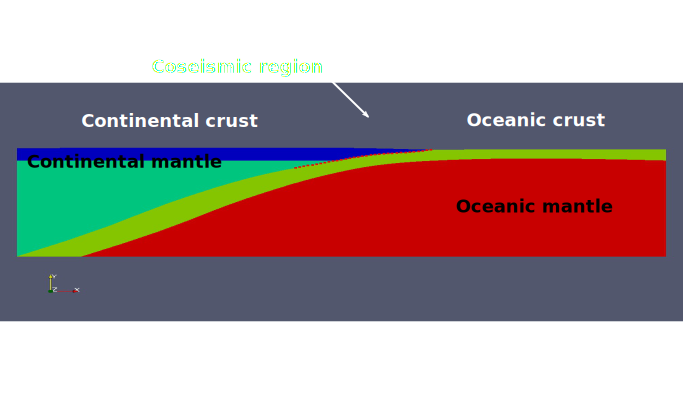
\includegraphics[width=4.5in]{figs/subduction2d_mesh}
  \end{center}
  \vfill

\end{frame}


% ========================================================== SECTION
\subsection{3D Example}

% ------------------------------------------------------------ SLIDE
\begin{frame}
  \frametitle{3D Subduction Zone}
  \summary{Mesh with subduction thrust, splay fault, and topo/bathymetry}
 
  \vfill
  \begin{center}
    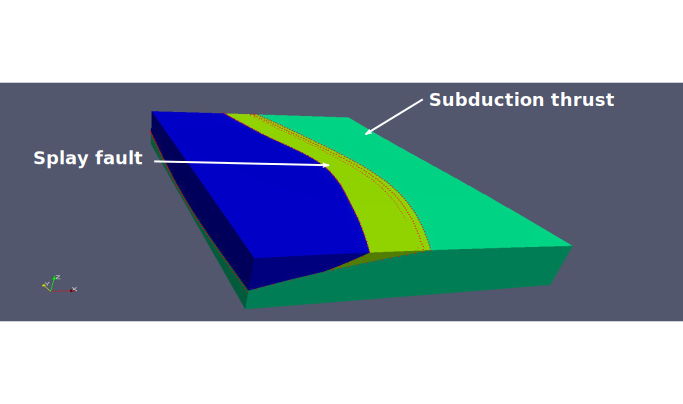
\includegraphics[width=4.5in]{figs/subduction3d_mesh}
  \end{center}
  \vfill

\end{frame}


% ========================================================== SECTION
\subsection{CUBIT Sizing Function}

% ------------------------------------------------------------ SLIDE
\begin{frame}
  \frametitle{Using user-defined fields to control mesh size}
  \summary{Example 1:   Use a spatial database to control cell size}
 
  \vfill
  \begin{center}
    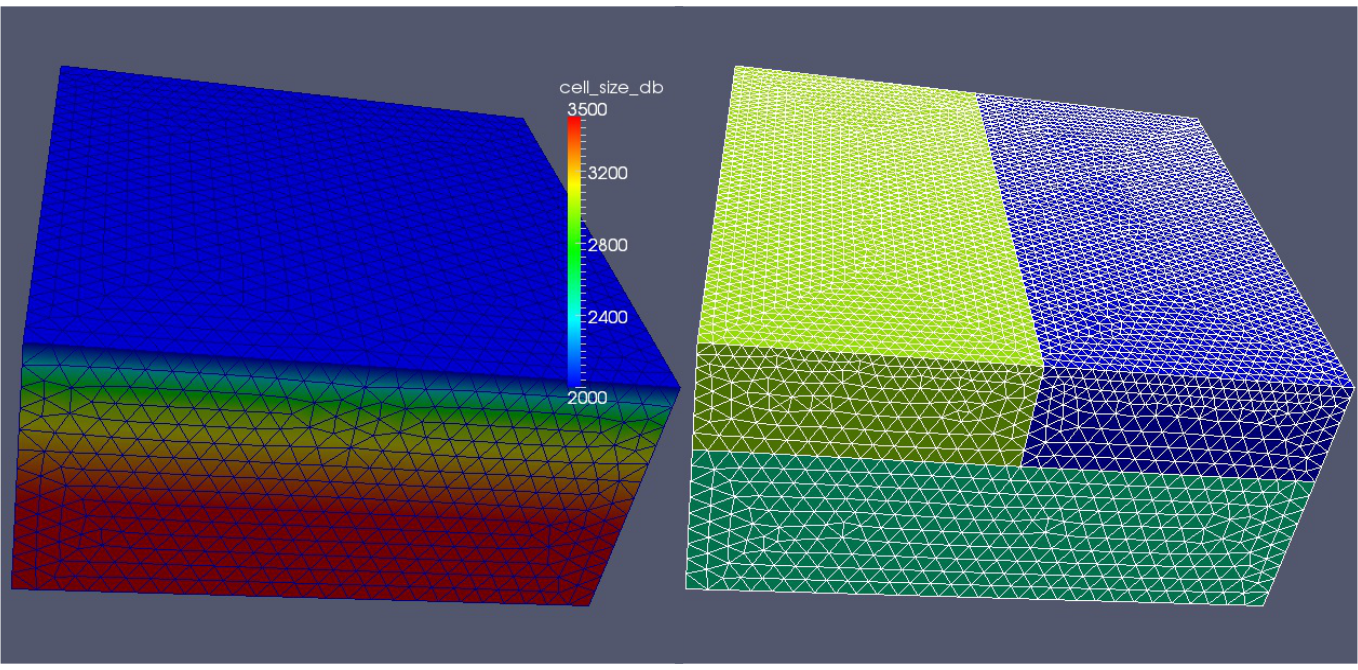
\includegraphics[width=4.5in]{figs/cellsize_mesh_spatialdb}
  \end{center}
  \vfill
 
\end{frame}


% ------------------------------------------------------------ SLIDE
\begin{frame}
  \frametitle{Using user-defined fields to control mesh size}
  \summary{Example 2:   Use an analytical function to control cell size}
 
  \vfill
  \begin{center}
    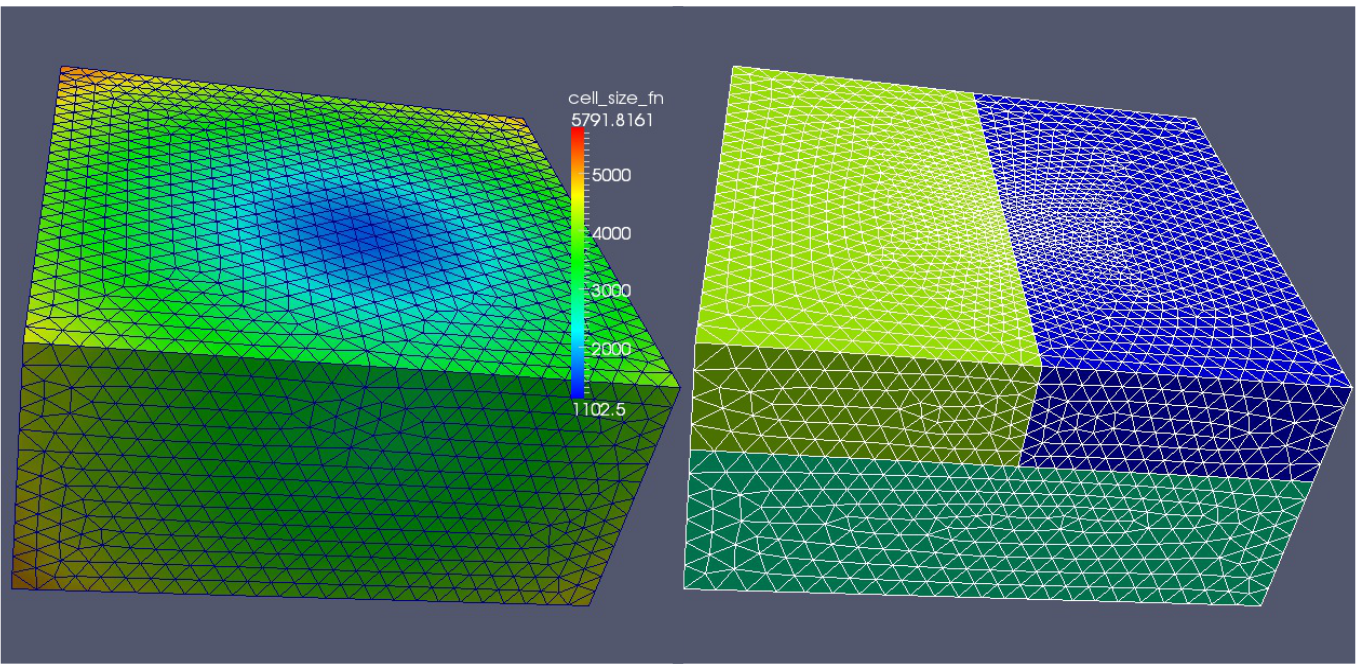
\includegraphics[width=4.5in]{figs/cellsize_mesh_analyticfn}
  \end{center}
  \vfill
 
\end{frame}
 

% ======================================================================
\end{document}


% End of file
